\documentclass[]{article}
\usepackage{lmodern}
\usepackage{amssymb,amsmath}
\usepackage{ifxetex,ifluatex}
\usepackage{fixltx2e} % provides \textsubscript
\ifnum 0\ifxetex 1\fi\ifluatex 1\fi=0 % if pdftex
  \usepackage[T1]{fontenc}
  \usepackage[utf8]{inputenc}
\else % if luatex or xelatex
  \ifxetex
    \usepackage{mathspec}
  \else
    \usepackage{fontspec}
  \fi
  \defaultfontfeatures{Ligatures=TeX,Scale=MatchLowercase}
\fi
% use upquote if available, for straight quotes in verbatim environments
\IfFileExists{upquote.sty}{\usepackage{upquote}}{}
% use microtype if available
\IfFileExists{microtype.sty}{%
\usepackage[]{microtype}
\UseMicrotypeSet[protrusion]{basicmath} % disable protrusion for tt fonts
}{}
\PassOptionsToPackage{hyphens}{url} % url is loaded by hyperref
\usepackage[unicode=true]{hyperref}
\hypersetup{
            pdftitle={Minimum Viable Analysis},
            pdfauthor={R Ju},
            pdfborder={0 0 0},
            breaklinks=true}
\urlstyle{same}  % don't use monospace font for urls
\usepackage[margin=1in]{geometry}
\usepackage{color}
\usepackage{fancyvrb}
\newcommand{\VerbBar}{|}
\newcommand{\VERB}{\Verb[commandchars=\\\{\}]}
\DefineVerbatimEnvironment{Highlighting}{Verbatim}{commandchars=\\\{\}}
% Add ',fontsize=\small' for more characters per line
\usepackage{framed}
\definecolor{shadecolor}{RGB}{248,248,248}
\newenvironment{Shaded}{\begin{snugshade}}{\end{snugshade}}
\newcommand{\KeywordTok}[1]{\textcolor[rgb]{0.13,0.29,0.53}{\textbf{#1}}}
\newcommand{\DataTypeTok}[1]{\textcolor[rgb]{0.13,0.29,0.53}{#1}}
\newcommand{\DecValTok}[1]{\textcolor[rgb]{0.00,0.00,0.81}{#1}}
\newcommand{\BaseNTok}[1]{\textcolor[rgb]{0.00,0.00,0.81}{#1}}
\newcommand{\FloatTok}[1]{\textcolor[rgb]{0.00,0.00,0.81}{#1}}
\newcommand{\ConstantTok}[1]{\textcolor[rgb]{0.00,0.00,0.00}{#1}}
\newcommand{\CharTok}[1]{\textcolor[rgb]{0.31,0.60,0.02}{#1}}
\newcommand{\SpecialCharTok}[1]{\textcolor[rgb]{0.00,0.00,0.00}{#1}}
\newcommand{\StringTok}[1]{\textcolor[rgb]{0.31,0.60,0.02}{#1}}
\newcommand{\VerbatimStringTok}[1]{\textcolor[rgb]{0.31,0.60,0.02}{#1}}
\newcommand{\SpecialStringTok}[1]{\textcolor[rgb]{0.31,0.60,0.02}{#1}}
\newcommand{\ImportTok}[1]{#1}
\newcommand{\CommentTok}[1]{\textcolor[rgb]{0.56,0.35,0.01}{\textit{#1}}}
\newcommand{\DocumentationTok}[1]{\textcolor[rgb]{0.56,0.35,0.01}{\textbf{\textit{#1}}}}
\newcommand{\AnnotationTok}[1]{\textcolor[rgb]{0.56,0.35,0.01}{\textbf{\textit{#1}}}}
\newcommand{\CommentVarTok}[1]{\textcolor[rgb]{0.56,0.35,0.01}{\textbf{\textit{#1}}}}
\newcommand{\OtherTok}[1]{\textcolor[rgb]{0.56,0.35,0.01}{#1}}
\newcommand{\FunctionTok}[1]{\textcolor[rgb]{0.00,0.00,0.00}{#1}}
\newcommand{\VariableTok}[1]{\textcolor[rgb]{0.00,0.00,0.00}{#1}}
\newcommand{\ControlFlowTok}[1]{\textcolor[rgb]{0.13,0.29,0.53}{\textbf{#1}}}
\newcommand{\OperatorTok}[1]{\textcolor[rgb]{0.81,0.36,0.00}{\textbf{#1}}}
\newcommand{\BuiltInTok}[1]{#1}
\newcommand{\ExtensionTok}[1]{#1}
\newcommand{\PreprocessorTok}[1]{\textcolor[rgb]{0.56,0.35,0.01}{\textit{#1}}}
\newcommand{\AttributeTok}[1]{\textcolor[rgb]{0.77,0.63,0.00}{#1}}
\newcommand{\RegionMarkerTok}[1]{#1}
\newcommand{\InformationTok}[1]{\textcolor[rgb]{0.56,0.35,0.01}{\textbf{\textit{#1}}}}
\newcommand{\WarningTok}[1]{\textcolor[rgb]{0.56,0.35,0.01}{\textbf{\textit{#1}}}}
\newcommand{\AlertTok}[1]{\textcolor[rgb]{0.94,0.16,0.16}{#1}}
\newcommand{\ErrorTok}[1]{\textcolor[rgb]{0.64,0.00,0.00}{\textbf{#1}}}
\newcommand{\NormalTok}[1]{#1}
\usepackage{graphicx,grffile}
\makeatletter
\def\maxwidth{\ifdim\Gin@nat@width>\linewidth\linewidth\else\Gin@nat@width\fi}
\def\maxheight{\ifdim\Gin@nat@height>\textheight\textheight\else\Gin@nat@height\fi}
\makeatother
% Scale images if necessary, so that they will not overflow the page
% margins by default, and it is still possible to overwrite the defaults
% using explicit options in \includegraphics[width, height, ...]{}
\setkeys{Gin}{width=\maxwidth,height=\maxheight,keepaspectratio}
\IfFileExists{parskip.sty}{%
\usepackage{parskip}
}{% else
\setlength{\parindent}{0pt}
\setlength{\parskip}{6pt plus 2pt minus 1pt}
}
\setlength{\emergencystretch}{3em}  % prevent overfull lines
\providecommand{\tightlist}{%
  \setlength{\itemsep}{0pt}\setlength{\parskip}{0pt}}
\setcounter{secnumdepth}{0}
% Redefines (sub)paragraphs to behave more like sections
\ifx\paragraph\undefined\else
\let\oldparagraph\paragraph
\renewcommand{\paragraph}[1]{\oldparagraph{#1}\mbox{}}
\fi
\ifx\subparagraph\undefined\else
\let\oldsubparagraph\subparagraph
\renewcommand{\subparagraph}[1]{\oldsubparagraph{#1}\mbox{}}
\fi

% set default figure placement to htbp
\makeatletter
\def\fps@figure{htbp}
\makeatother


\title{Minimum Viable Analysis}
\author{R Ju}
\date{10/22/2020}

\begin{document}
\maketitle

\subsection{Data collection}\label{data-collection}

To begin, I will compile a list of known Symbiodinium clade associations
for species within the genus \emph{Porites} from \url{coraltraits.org}.
This is an abundant and widespread genus of scleractinian corals. Data
downloaded from this site also includes the geographic location of the
sample, as well as methodology used. These factors may be useful in
comparative analyses with a larger data set.

\begin{Shaded}
\begin{Highlighting}[]
\CommentTok{#load in coraltraits.org data and filter for relevant species and trait}
\NormalTok{por_sym <-}\StringTok{ }\KeywordTok{read.csv}\NormalTok{(}\StringTok{"data/ctdb_1.1.0_data.csv"}\NormalTok{) }\OperatorTok
\StringTok{  }\KeywordTok{filter}\NormalTok{(trait_name }\OperatorTok{==}\StringTok{ "Symbiodinium clade"} \OperatorTok{&}\StringTok{ }\KeywordTok{str_detect}\NormalTok{(specie_name, }\StringTok{"Porites"}\NormalTok{)) }\OperatorTok
\StringTok{  }\KeywordTok{select}\NormalTok{(specie_id, specie_name, location_id, location_name, trait_id, trait_name, methodology_id, methodology_name, value)}

\CommentTok{#visualize data (Symbiodinium clades by species)}
\KeywordTok{ggplot}\NormalTok{(por_sym) }\OperatorTok{+}
\StringTok{  }\KeywordTok{geom_bar}\NormalTok{(}\KeywordTok{aes}\NormalTok{(}\DataTypeTok{x =}\NormalTok{ value, }\DataTypeTok{fill =}\NormalTok{ value)) }\OperatorTok{+}\StringTok{ }
\StringTok{  }\KeywordTok{facet_wrap}\NormalTok{(}\OperatorTok{~}\NormalTok{specie_name) }\OperatorTok{+}\StringTok{ }
\StringTok{  }\KeywordTok{labs}\NormalTok{(}\DataTypeTok{x =} \StringTok{'Symbiodinium clade'}\NormalTok{,}
       \DataTypeTok{y =} \StringTok{'Observations'}\NormalTok{) }\OperatorTok{+}
\StringTok{  }\KeywordTok{scale_fill_manual}\NormalTok{(}\DataTypeTok{breaks =} \KeywordTok{c}\NormalTok{(}\StringTok{"C"}\NormalTok{, }\StringTok{"B"}\NormalTok{, }\StringTok{"A"}\NormalTok{, }\StringTok{"F"}\NormalTok{), }\DataTypeTok{values =} \KeywordTok{c}\NormalTok{(}\StringTok{"tomato"}\NormalTok{, }\StringTok{"cornflowerblue"}\NormalTok{, }\StringTok{"seagreen2"}\NormalTok{, }\StringTok{"gold"}\NormalTok{), }\DataTypeTok{name =} \StringTok{"Symbiodinium clade"}\NormalTok{) }\OperatorTok{+}\StringTok{ }
\StringTok{  }\KeywordTok{theme_bw}\NormalTok{() }\OperatorTok{+}\StringTok{ }\KeywordTok{theme}\NormalTok{(}\DataTypeTok{panel.border =} \KeywordTok{element_rect}\NormalTok{(}\DataTypeTok{color=}\StringTok{"black"}\NormalTok{, }\DataTypeTok{fill=}\OtherTok{NA}\NormalTok{, }\DataTypeTok{size=}\FloatTok{0.75}\NormalTok{), }\DataTypeTok{panel.grid.major =} \KeywordTok{element_blank}\NormalTok{(),}
                     \DataTypeTok{panel.grid.minor =} \KeywordTok{element_blank}\NormalTok{(), }\DataTypeTok{axis.line =} \KeywordTok{element_blank}\NormalTok{()) }
\end{Highlighting}
\end{Shaded}

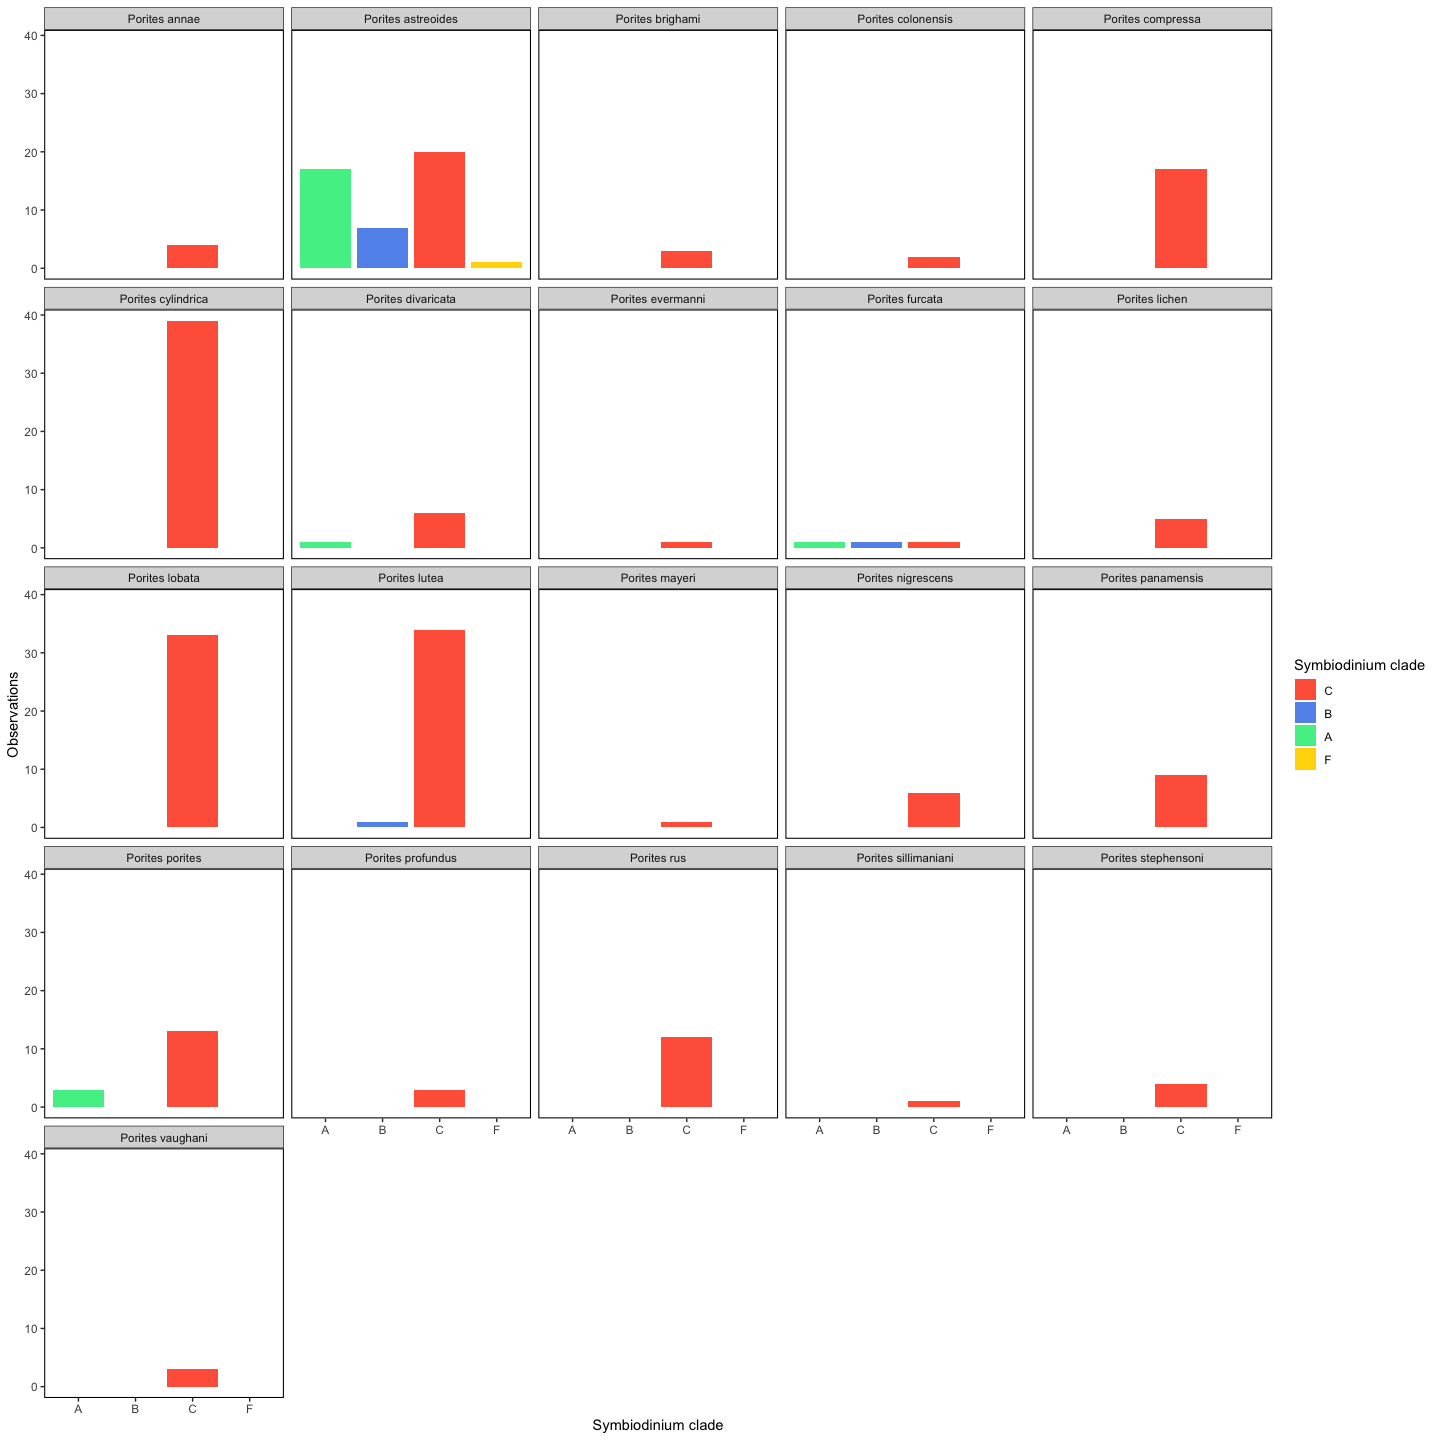
\includegraphics{min_via_analysis_files/figure-latex/data clean-1.pdf}

Four different \emph{Symbiodinium} clades are found in the genus
\emph{Porites}. However, we see that clade C is dominant across most
species. Additionally, there is wide variation between the number of
observations for each species. This could lead to trouble later on, so
in future analyses it may be worth investigating other data sources.

To better see the different \emph{Symbiodinium} associations for each
species, we can also plot pie graphs representing the proportion of the
total number of observations attributed to each clade.

\begin{Shaded}
\begin{Highlighting}[]
\CommentTok{#visualize proportion data}
\NormalTok{por_sym_prop <-}\StringTok{ }\NormalTok{por_sym }\OperatorTok
\StringTok{  }\KeywordTok{count}\NormalTok{(specie_name, value) }\OperatorTok
\StringTok{  }\KeywordTok{group_by}\NormalTok{(specie_name) }\OperatorTok
\StringTok{  }\KeywordTok{mutate}\NormalTok{(}\DataTypeTok{prop =} \KeywordTok{prop.table}\NormalTok{(n)) }\CommentTok{#saves prop table of symbiodinium clade by species}
\NormalTok{por_sym_prop }\OperatorTok
\StringTok{  }\KeywordTok{ggplot}\NormalTok{(}\KeywordTok{aes}\NormalTok{(}\DataTypeTok{x =} \StringTok{""}\NormalTok{, }\DataTypeTok{y =}\NormalTok{ prop, }\DataTypeTok{fill =}\NormalTok{ value), }\DataTypeTok{size =} \DecValTok{12}\NormalTok{) }\OperatorTok{+}
\StringTok{  }\KeywordTok{geom_bar}\NormalTok{(}\DataTypeTok{stat =} \StringTok{"identity"}\NormalTok{, }\DataTypeTok{width =} \FloatTok{0.5}\NormalTok{, }\DataTypeTok{color =} \StringTok{"white"}\NormalTok{) }\OperatorTok{+}\StringTok{ }
\StringTok{  }\KeywordTok{coord_polar}\NormalTok{(}\StringTok{"y"}\NormalTok{, }\DataTypeTok{start=}\DecValTok{0}\NormalTok{) }\OperatorTok{+}
\StringTok{  }\KeywordTok{scale_fill_manual}\NormalTok{(}\DataTypeTok{breaks =} \KeywordTok{c}\NormalTok{(}\StringTok{"C"}\NormalTok{, }\StringTok{"B"}\NormalTok{, }\StringTok{"A"}\NormalTok{, }\StringTok{"F"}\NormalTok{), }\DataTypeTok{values =} \KeywordTok{c}\NormalTok{(}\StringTok{"tomato"}\NormalTok{, }\StringTok{"cornflowerblue"}\NormalTok{, }\StringTok{"seagreen2"}\NormalTok{, }\StringTok{"gold"}\NormalTok{), }\DataTypeTok{name =} \StringTok{"Symbiodinium clade"}\NormalTok{) }\OperatorTok{+}\StringTok{ }
\StringTok{  }\KeywordTok{facet_wrap}\NormalTok{(}\OperatorTok{~}\NormalTok{specie_name) }\OperatorTok{+}\StringTok{ }
\StringTok{  }\KeywordTok{theme_void}\NormalTok{()}
\end{Highlighting}
\end{Shaded}

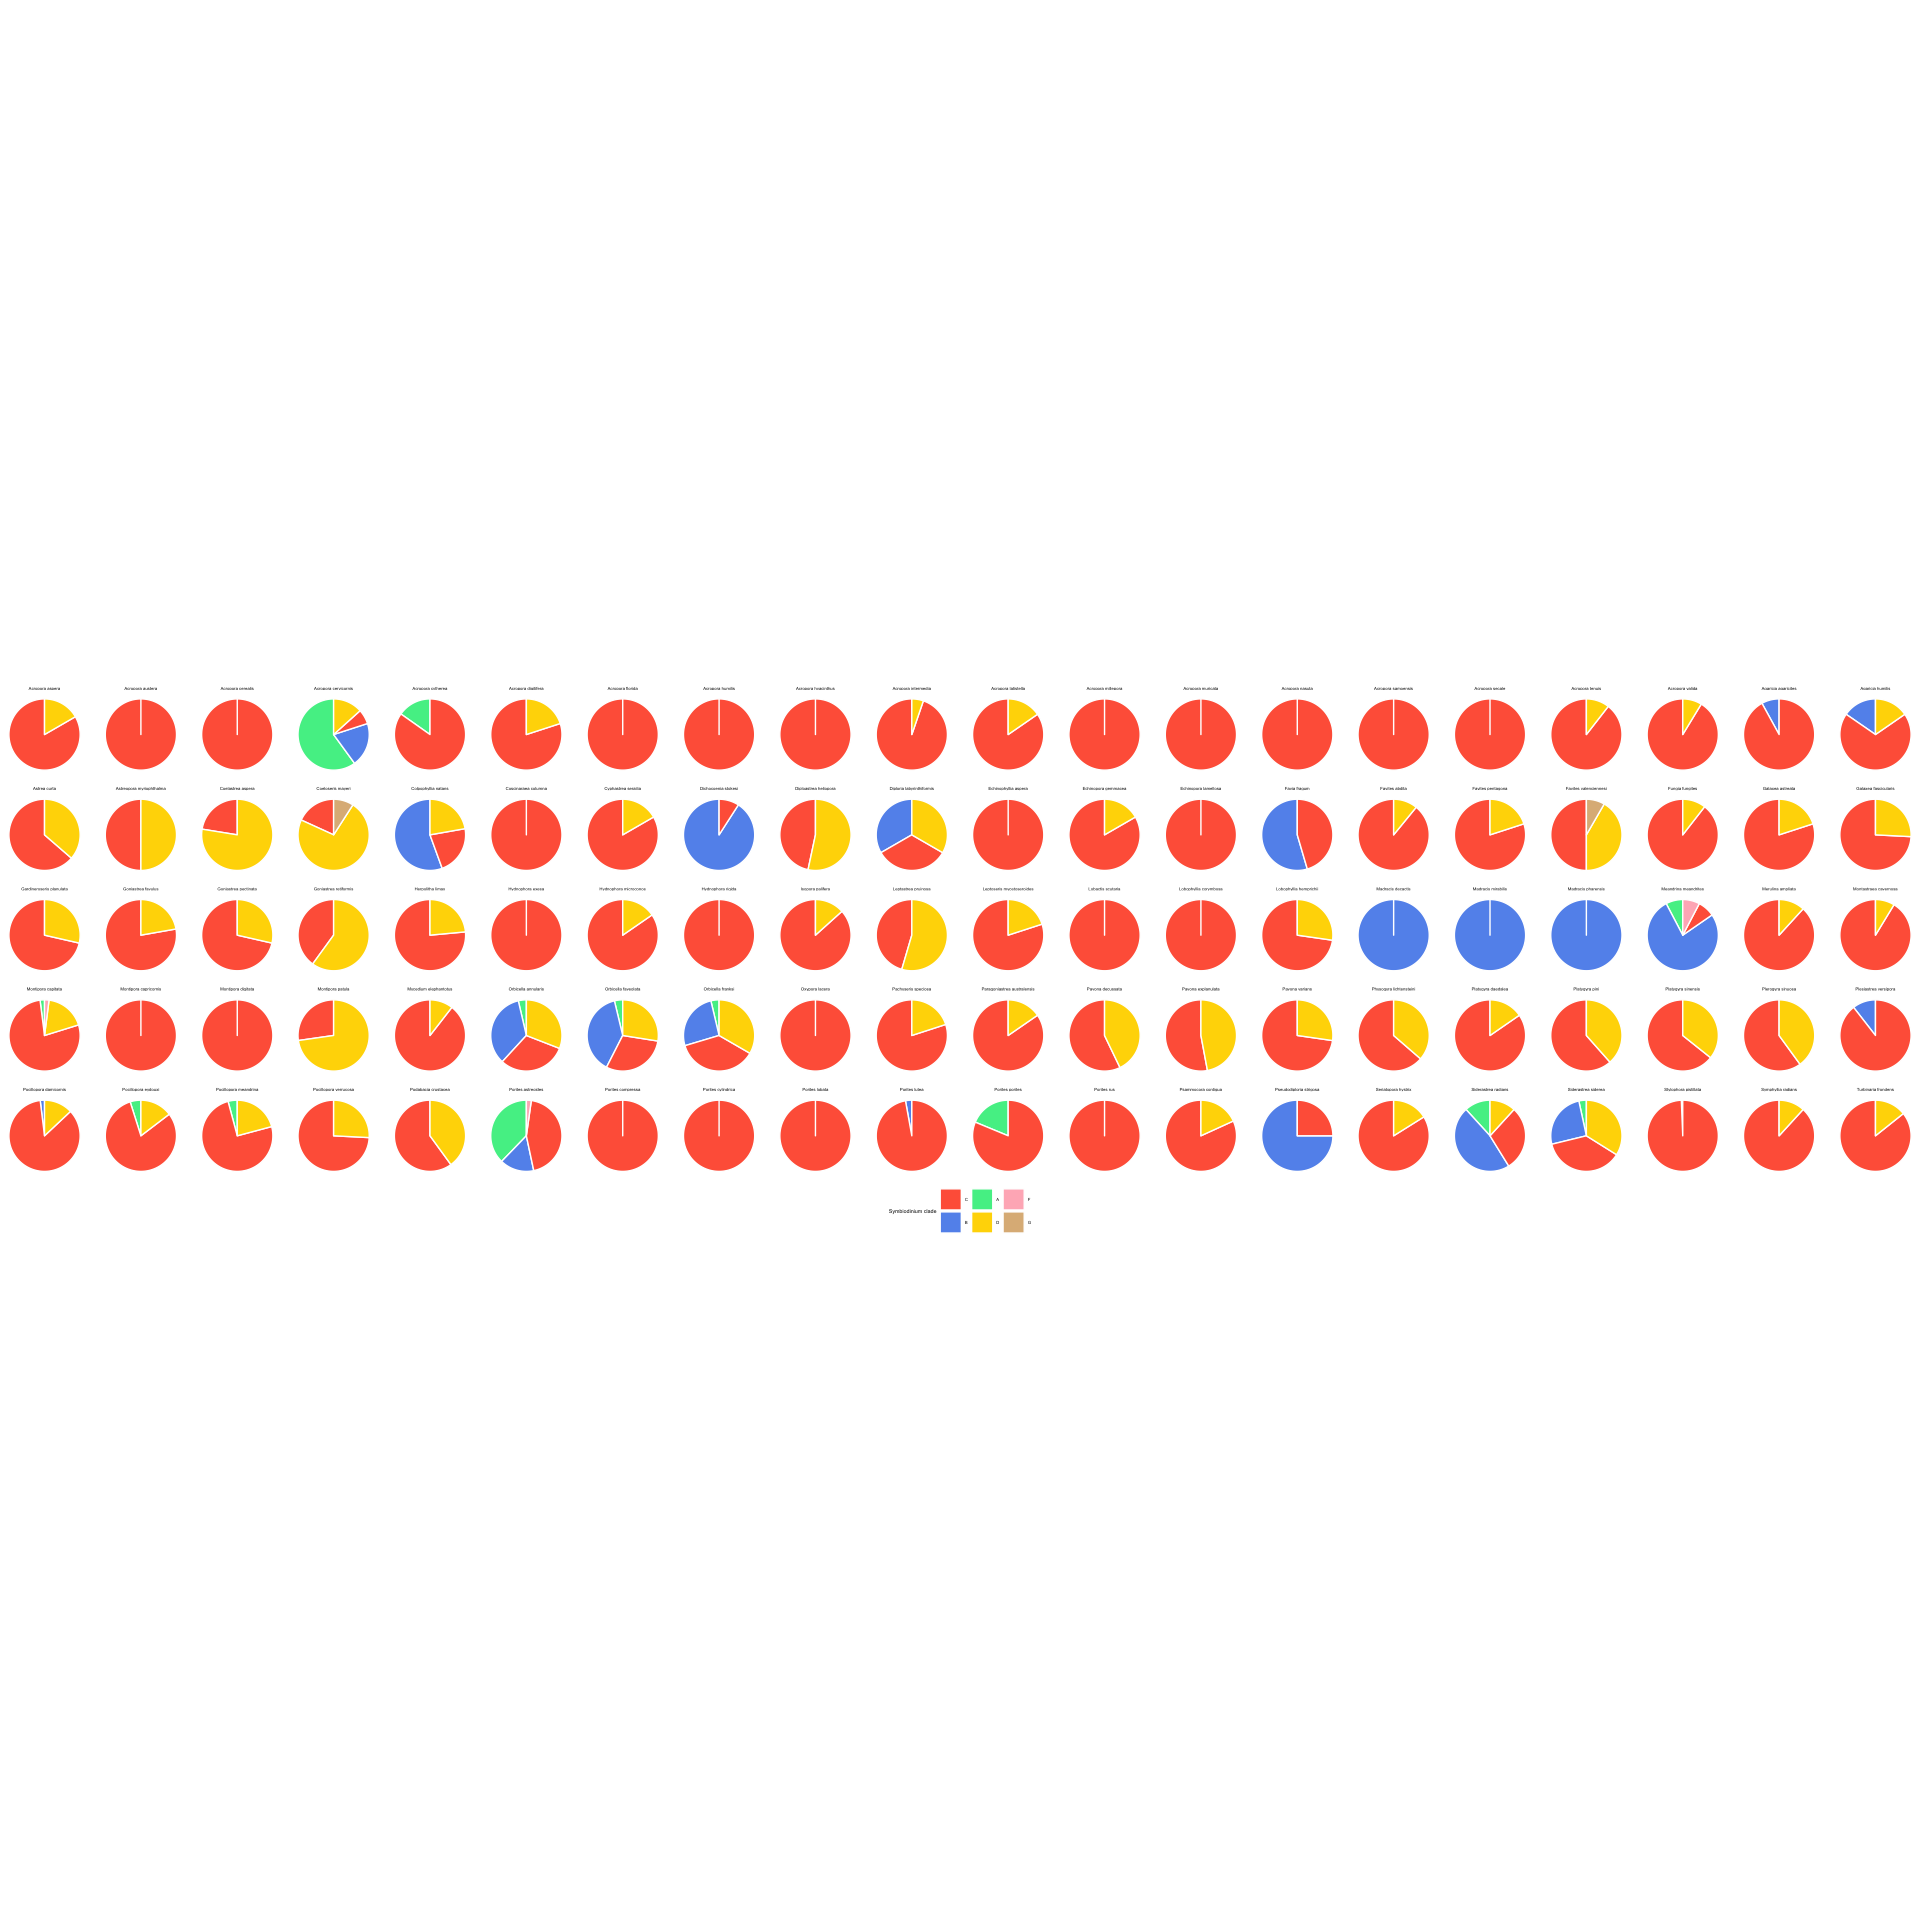
\includegraphics{min_via_analysis_files/figure-latex/unnamed-chunk-1-1.pdf}

Again, it is clear that clade C is dominant, as it is observed in every
species. However, five species also were found to associate with other
clades. For this initial analysis, the goal will be to map these
observations to a phylogenetic tree, and examine if there is evidence
that associations with non-C clade \emph{Symbiodinium} are conserved
phylogenetically.

Subsequent analyses may yield a far more diverse assortment of
\emph{Symbiodinium} associations --- this initial glance suggests that
clade association may be consistent across genera. It will certainly be
interesting to expand the data set, as well as to examine the effects of
other factors such as geographical location on clade association.

\subsection{Phylogenetic inference}\label{phylogenetic-inference}

For this analysis, I will build a tree using just the CO1 (cytochrome c
oxydase 1) gene. The scleractinian coral species \emph{Siderastrea
siderea} will serve as the outgroup. As this project continues, I will
gather additional gene sequences to use in the phylogenetic inference,
and refine the outgroup choice as needed.

Clade name: Porites (taxid: 46719)

Outgroup: Siderastrea siderea (taxid: 130672)

Bait sequence:

\begin{verbatim}
>HM754452.1 Palythoa cf. heliodiscus SMH-2011 isolate 305.11.2 cytochrome oxidase subunit I (CO1) gene, partial cds; mitochondrial
  CAGGTAAACTTCAGGGTGACCAAAAAATCAAAAGAGATGTTGAAACAGAATCGGGTCCCCCCCTCCGGCG
  GGGTCAAAGAAAGTAGTGTTAAAATTCCTATCTGTCAACAGCATGGTTATAGCCCCGGCCAATACGGGCA
  AAGACAGTAACAATAAGAAGGCGGTGATTAAGATAGACCACACAAAGAGTGGCAATCTATCCATTGTCAT
  ACCCGGGGCCCTCATATTAAATATAGTGGTGATAAAATTCATAGCCCCTAAGATGGAAGAGACCCCGGCC
  AAGTGGAGGCTAAATATAACCATGTCCACGGCCCCCCCCGAATGAGCTTGAATGGCTGAAAGAGGCGGAT
  ACACCGTCCAACCTGTTCCTGCCCCCTGTTCCACAAAGGCGGAACCCAACAATAGAATTAGGGCGGGGGG
  CAAGAGCCAGAAACTAATGTTATTTAGTCGCGGGAAGGCCATATCTGGTGCACCGATATATAGCGGCACC
  AACCAATTCCCAAACCCCCCTATCATCACCGGCATCACCAGGAAAAAGATCATAACAAAAGCATGCGCAG
  TCACGATTACATTATAAAGATGGTCGTCCCCCAACATAGTTCCGGGAGCAGAAAGTTCTAACCTTATCAA
  CATACTGAAAGCTGTTCCTATCATACCGGCCCCAACACCAAATATTAGATATAATGTGCCAATATCTTTA
  TGATTTGTTGACCGTCGTTT
\end{verbatim}

Phylogeny was inferred using IQ-TREE and the cluster. Bootstrap analyses
were conducted to determine support values for the resulting tree.
Further work will compare models as well as use Bayesian analyses to
determine phylogenetic topology.

Job script:

\begin{verbatim}
#!/bin/bash

#SBATCH --partition=eeb354
#SBATCH --job-name=clade_iqtree
#SBATCH --time=2:00:00
#SBATCH --ntasks=1
#SBATCH --cpus-per-task=8

module load IQ-TREE/1.6.12

iqtree -s por.co1.alignment.fasta -bb 1000 -nt AUTO
\end{verbatim}

The tips of this tree correspond to individual sequences, rather than
species. As such, visualization requires adjustment of the tip labels to
match the \emph{Symbiodinium} dataset. Some studies consolidate
sequences by species before building tree and mapping on the data, while
others do not. I think using multiple genes will force consolidation by
species, but this will become more complex when considering cryptic
speciation or unclassified samples. Ultimately, the goal is to ensure
that there is a 1:1 relationship between the \emph{Symbiodinium} samples
and the phylogenetic sequences.

\begin{Shaded}
\begin{Highlighting}[]
\CommentTok{#read in cluster output}
\NormalTok{por_phy <-}\StringTok{ }\KeywordTok{read.tree}\NormalTok{(}\StringTok{"cluster/por.co1.alignment.fasta.treefile"}\NormalTok{) }

\CommentTok{#clean up tip labels and manually correct erros}
\NormalTok{por_phy}\OperatorTok{$}\NormalTok{tip.label <-}\StringTok{ }\NormalTok{por_phy}\OperatorTok{$}\NormalTok{tip.label }\OperatorTok
\StringTok{  }\KeywordTok{str_replace_all}\NormalTok{(}\StringTok{"_"}\NormalTok{,}\StringTok{" "}\NormalTok{)}
\NormalTok{por_phy}\OperatorTok{$}\NormalTok{tip.label[}\DecValTok{2}\NormalTok{] <-}\StringTok{ "Porites harrisoni "} \CommentTok{#unsure why the sed line failed!}
\NormalTok{por_phy}\OperatorTok{$}\NormalTok{tip.label[}\DecValTok{62}\NormalTok{] <-}\StringTok{ "Porites fontanesii "}

\CommentTok{# por_phy$tip.label <- str_sub(por_phy$tip.label, end = sapply(str_locate_all(por_phy$tip.label," "), "[[", 2)-1)}

\CommentTok{#remove outgroup for easier plotting  }
\NormalTok{por_phy <-}\StringTok{ }\KeywordTok{drop.tip}\NormalTok{(por_phy, }\StringTok{"Siderastrea siderea AY451386.1"}\NormalTok{)}

\CommentTok{#plot tree with support values}
\KeywordTok{plot}\NormalTok{(por_phy) }\CommentTok{#maybe plot with ggtree? figure is messy and hard to read}
\KeywordTok{nodelabels}\NormalTok{(por_phy}\OperatorTok{$}\NormalTok{node.label)}
\end{Highlighting}
\end{Shaded}

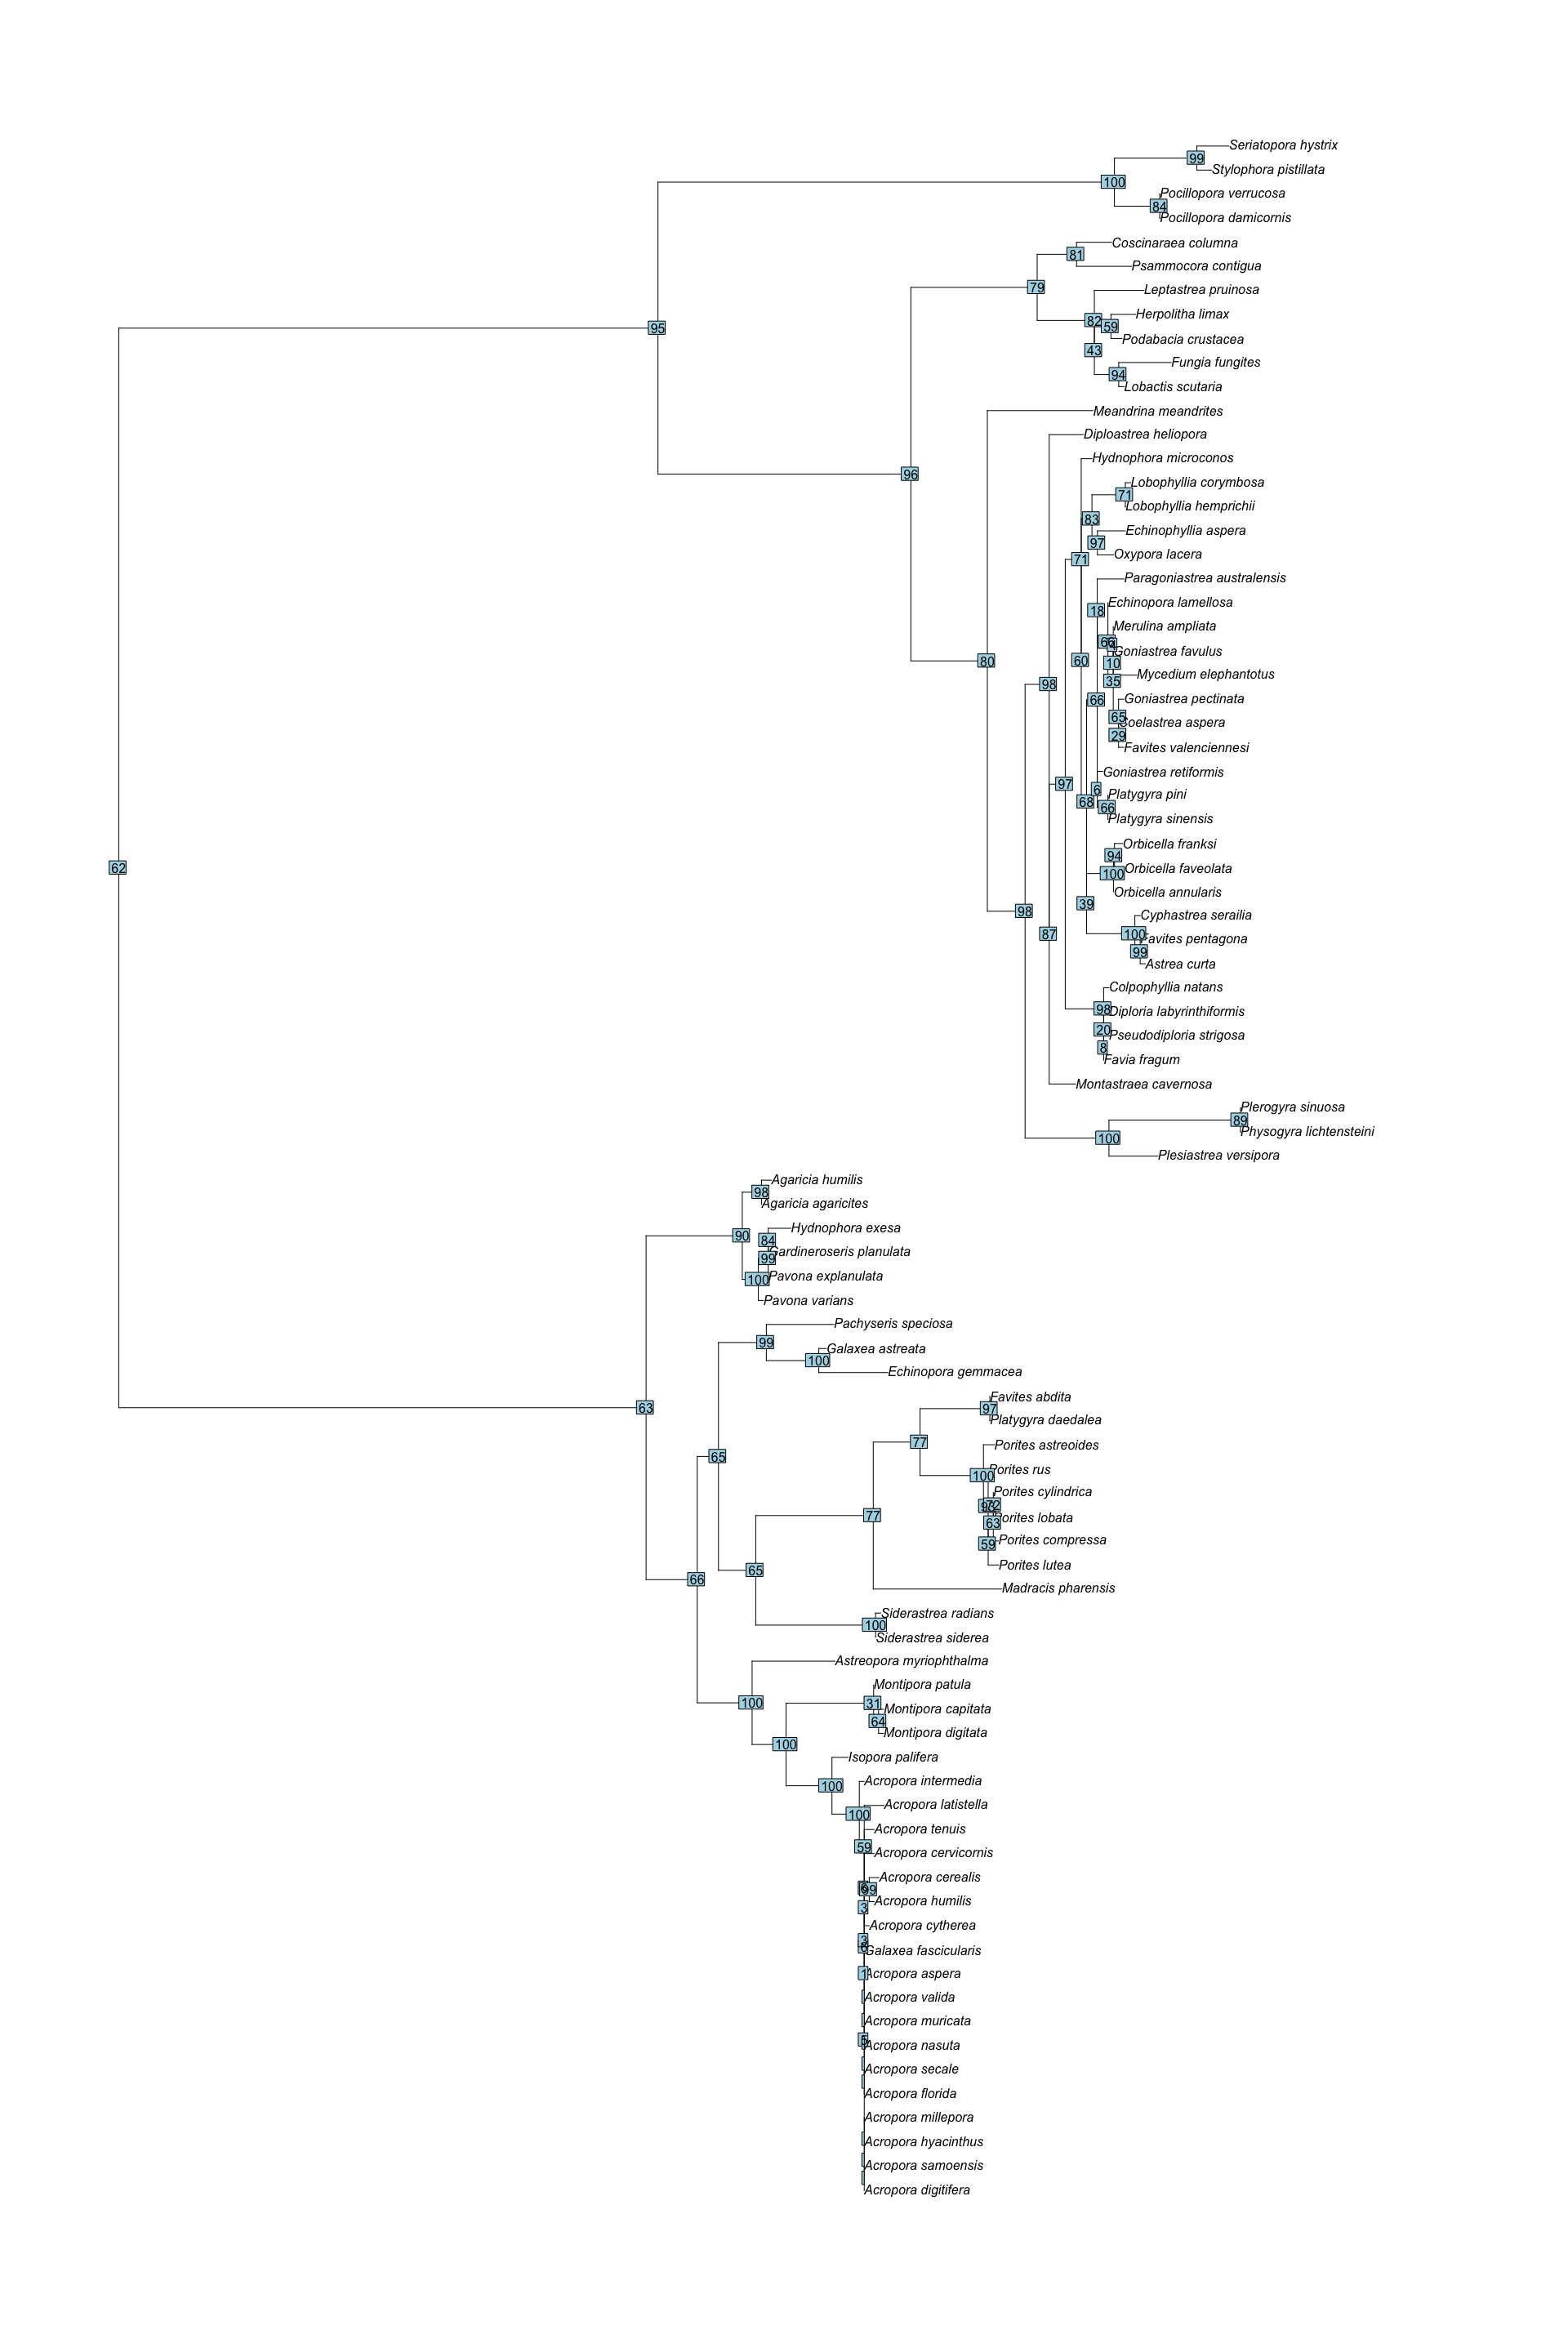
\includegraphics{min_via_analysis_files/figure-latex/unnamed-chunk-2-1.pdf}

There are definitely a few concerning things about this tree --- many of
the support values seem quite low, suggesting there is a better topology
that was not reached by this basic model. Additionally, sequences from
the same species are not always adjacent. These issues may be resolved
with additional data. Also, branch lengths and evolutionary time are not
as vital to my analysis. However, I'd like to investigate more as to why
there is such high variation in the branch lengths.

To assess if \emph{Symbiodinium} associations reflect phylogeny, I
mapped the observed clades onto the tips of the tree. (This actually
turned out to be obscenely difficult to do, and I'm still not happy with
the figure!) As I kept the individual sequences, there are repeat
species in this tree. However, I think it's useful to be able to see the
individual sequences, and the \emph{Symbiodinium} clades were mapped on
by observed/not observed, rather than by proportion/\# of observations.
I may change how they are mapped on once more data is included.

\begin{Shaded}
\begin{Highlighting}[]
\CommentTok{#create data set with symb clade and tip labels}
\NormalTok{tips <-}\StringTok{ }\KeywordTok{data.frame}\NormalTok{(}\DataTypeTok{tip.label=}\NormalTok{por_phy}\OperatorTok{$}\NormalTok{tip.label, }\DataTypeTok{specie_name=}\KeywordTok{str_sub}\NormalTok{(por_phy}\OperatorTok{$}\NormalTok{tip.label, }\DataTypeTok{end =} \KeywordTok{sapply}\NormalTok{(}\KeywordTok{str_locate_all}\NormalTok{(por_phy}\OperatorTok{$}\NormalTok{tip.label,}\StringTok{" "}\NormalTok{), }\StringTok{"[["}\NormalTok{, }\DecValTok{2}\NormalTok{)}\OperatorTok{-}\DecValTok{1}\NormalTok{))}

\NormalTok{syms <-}\StringTok{ }\KeywordTok{full_join}\NormalTok{(tips, por_sym_prop, }\DataTypeTok{by=}\StringTok{"specie_name"}\NormalTok{) }\OperatorTok
\StringTok{  }\KeywordTok{filter}\NormalTok{(}\KeywordTok{is.na}\NormalTok{(value) }\OperatorTok{==}\StringTok{ }\OtherTok{FALSE}\NormalTok{) }\OperatorTok
\StringTok{  }\KeywordTok{group_by}\NormalTok{(tip.label) }\OperatorTok
\StringTok{  }\NormalTok{dplyr}\OperatorTok{::}\KeywordTok{summarise}\NormalTok{(}\DataTypeTok{value =}\NormalTok{ value) }\OperatorTok
\StringTok{  }\KeywordTok{filter}\NormalTok{(}\KeywordTok{is.na}\NormalTok{(tip.label) }\OperatorTok{==}\StringTok{ }\OtherTok{FALSE}\NormalTok{) }\OperatorTok
\StringTok{  }\KeywordTok{pivot_wider}\NormalTok{(}\DataTypeTok{names_from =}\NormalTok{ value)}

\CommentTok{#plot cladogram}
\KeywordTok{ggtree}\NormalTok{(por_phy, }\DataTypeTok{branch.length =} \StringTok{"none"}\NormalTok{, }\DataTypeTok{size =} \DecValTok{1}\NormalTok{) }\OperatorTok\StringTok{ }\NormalTok{syms }\OperatorTok{+}
\StringTok{  }\KeywordTok{geom_tiplab}\NormalTok{(}\DataTypeTok{fontface =} \StringTok{"italic"}\NormalTok{, }\DataTypeTok{size =} \DecValTok{10}\NormalTok{, }\DataTypeTok{offset =} \FloatTok{0.2}\NormalTok{) }\OperatorTok{+}
\StringTok{  }\KeywordTok{geom_tippoint}\NormalTok{(}\KeywordTok{aes}\NormalTok{(}\DataTypeTok{color=}\NormalTok{F), }\DataTypeTok{size =} \DecValTok{8}\NormalTok{) }\OperatorTok{+}
\StringTok{  }\KeywordTok{geom_tippoint}\NormalTok{(}\KeywordTok{aes}\NormalTok{(}\DataTypeTok{color=}\NormalTok{A), }\DataTypeTok{size =} \DecValTok{8}\NormalTok{, }\DataTypeTok{position =} \KeywordTok{position_dodge}\NormalTok{(}\DataTypeTok{width =} \DecValTok{1}\NormalTok{)) }\OperatorTok{+}
\StringTok{  }\KeywordTok{geom_tippoint}\NormalTok{(}\KeywordTok{aes}\NormalTok{(}\DataTypeTok{color=}\NormalTok{B), }\DataTypeTok{size =} \DecValTok{8}\NormalTok{, }\DataTypeTok{position =} \KeywordTok{position_dodge}\NormalTok{(}\DataTypeTok{width =} \DecValTok{2}\NormalTok{)) }\OperatorTok{+}
\StringTok{  }\KeywordTok{geom_tippoint}\NormalTok{(}\KeywordTok{aes}\NormalTok{(}\DataTypeTok{color=}\NormalTok{C), }\DataTypeTok{size =} \DecValTok{8}\NormalTok{, }\DataTypeTok{position =} \KeywordTok{position_dodge}\NormalTok{(}\DataTypeTok{width =} \DecValTok{3}\NormalTok{)) }\OperatorTok{+}
\StringTok{  }\KeywordTok{scale_color_manual}\NormalTok{(}\DataTypeTok{breaks =} \KeywordTok{c}\NormalTok{(}\StringTok{"C"}\NormalTok{, }\StringTok{"B"}\NormalTok{, }\StringTok{"A"}\NormalTok{, }\StringTok{"F"}\NormalTok{), }\DataTypeTok{values =} \KeywordTok{c}\NormalTok{(}\StringTok{"tomato"}\NormalTok{, }\StringTok{"cornflowerblue"}\NormalTok{, }\StringTok{"seagreen2"}\NormalTok{, }\StringTok{"gold"}\NormalTok{), }\DataTypeTok{name =} \StringTok{"Symbiodinium clade"}\NormalTok{) }\OperatorTok{+}\StringTok{ }
\StringTok{  }\KeywordTok{xlim}\NormalTok{(}\OperatorTok{-}\DecValTok{2}\NormalTok{, }\DecValTok{40}\NormalTok{) }\OperatorTok{+}\StringTok{ }
\StringTok{  }\KeywordTok{theme}\NormalTok{(}\DataTypeTok{legend.position =} \StringTok{"bottom"}\NormalTok{)}
\end{Highlighting}
\end{Shaded}

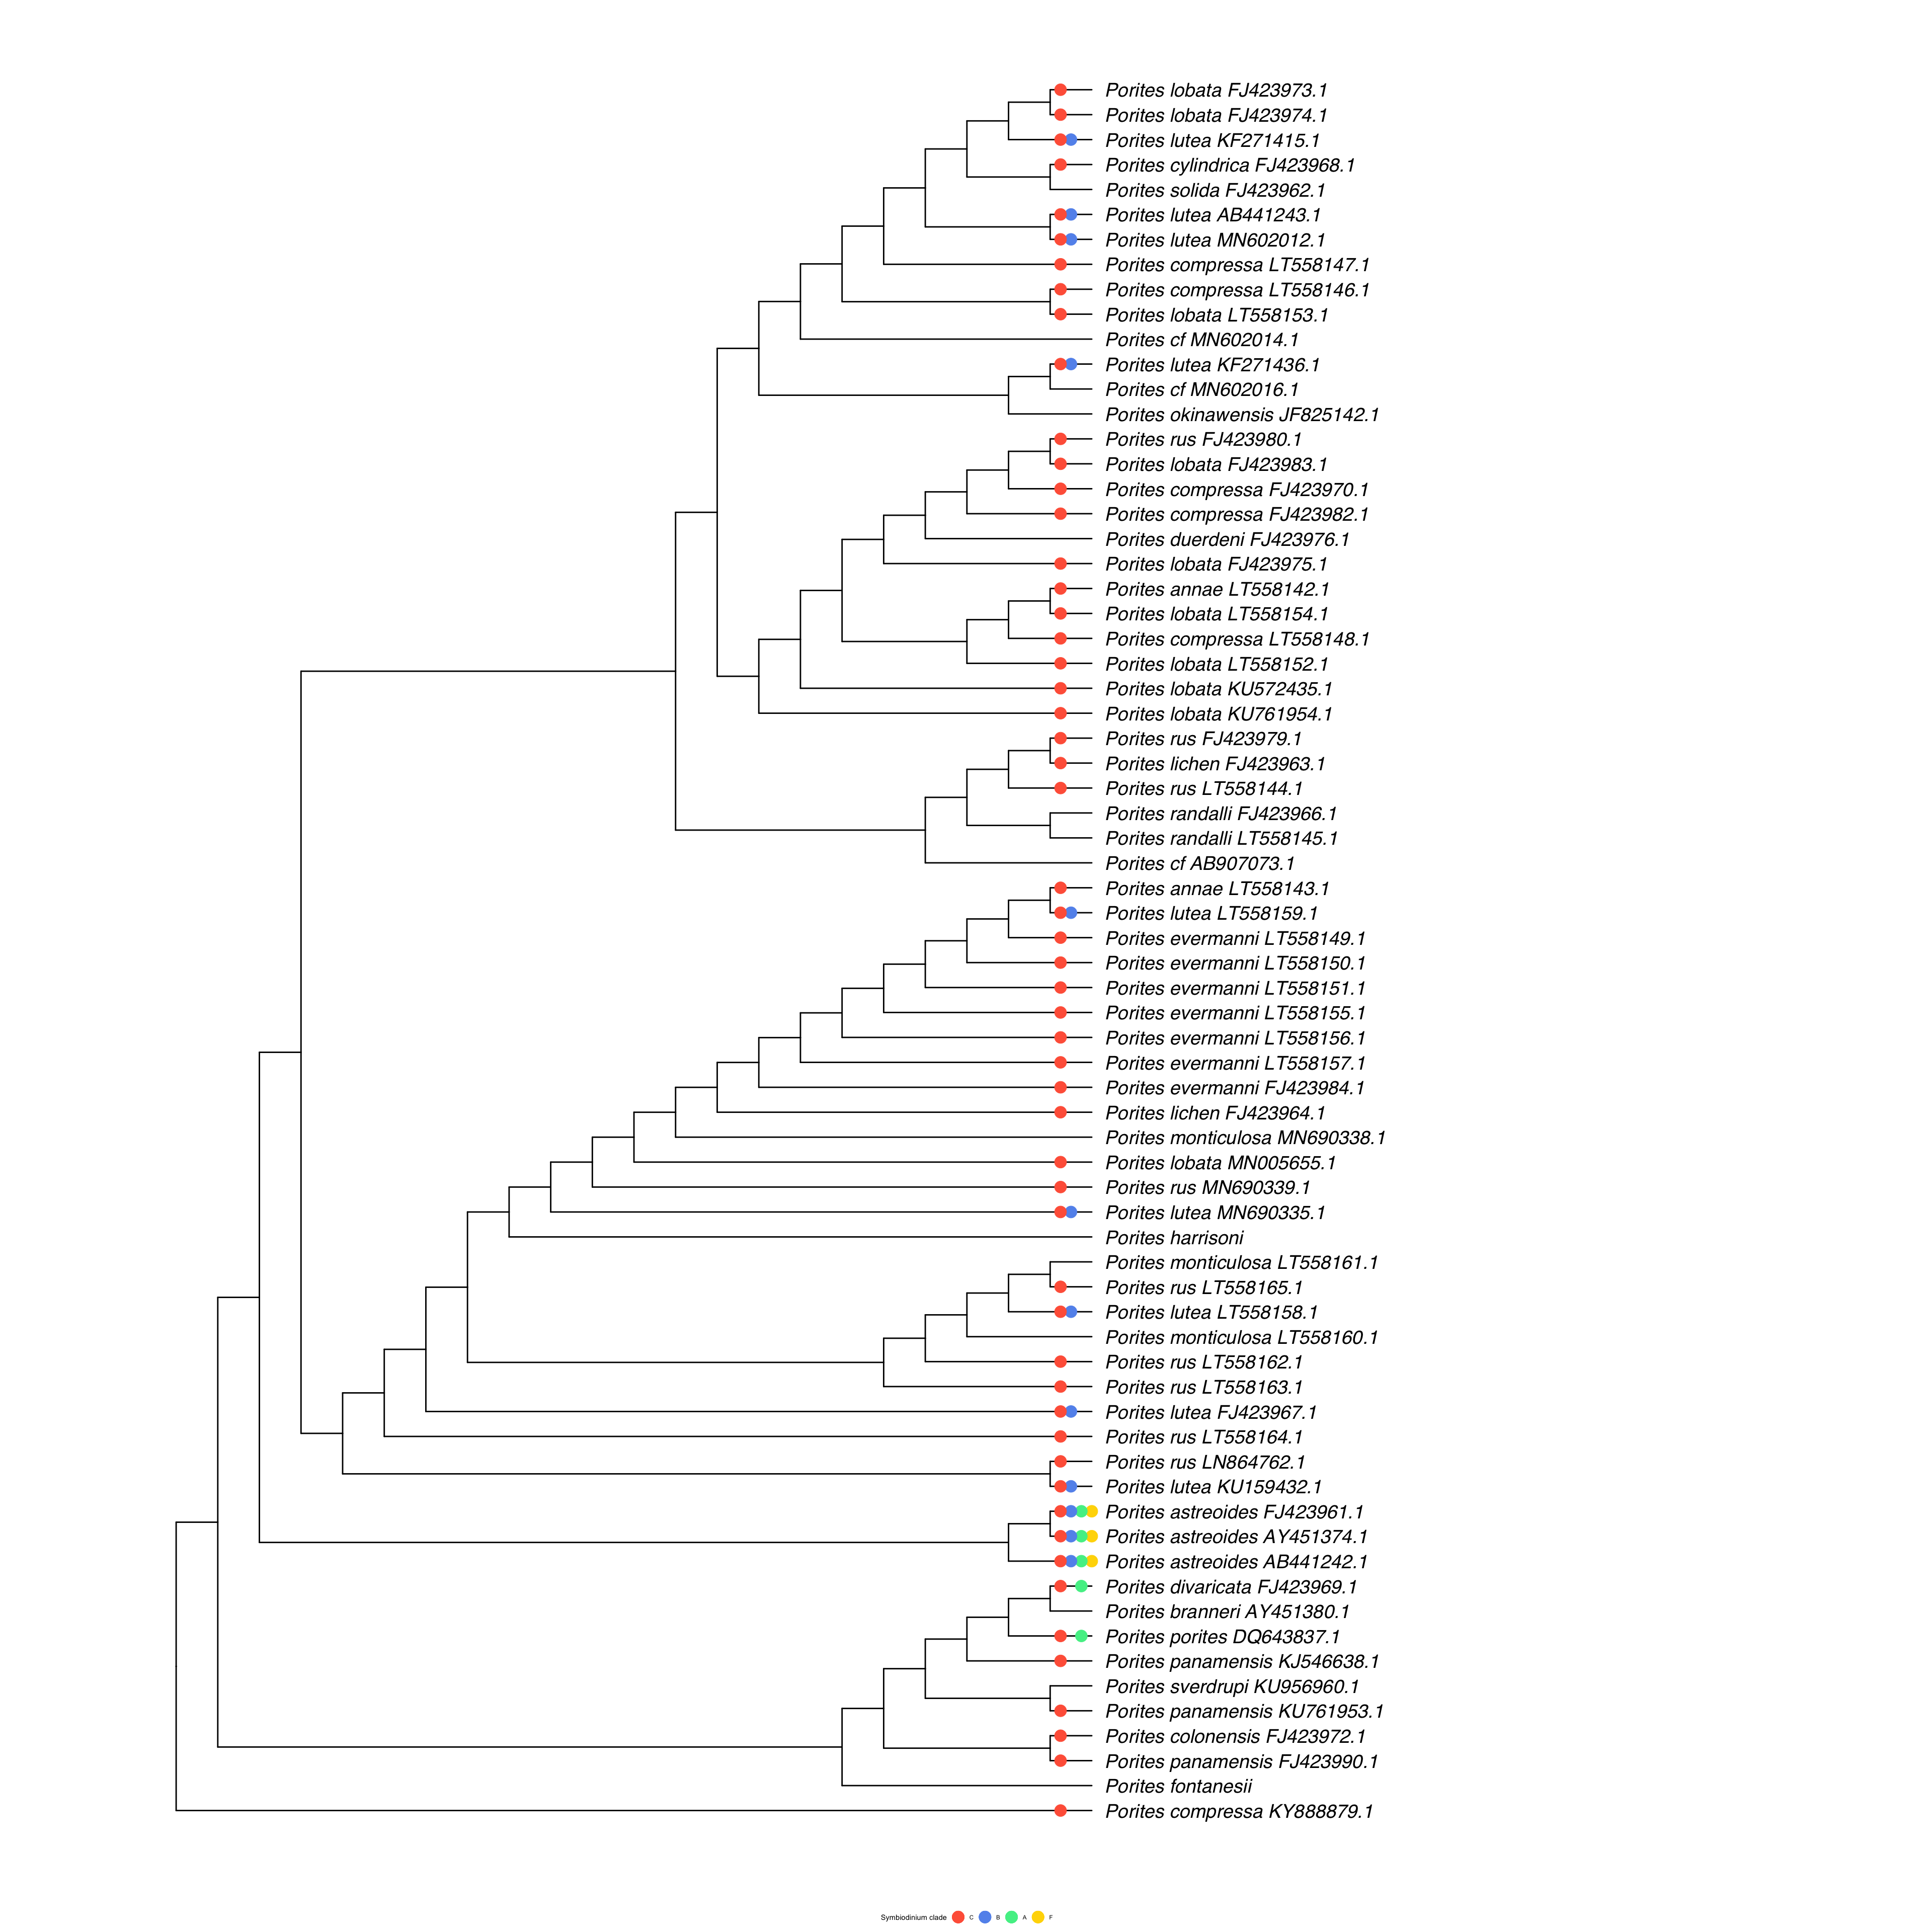
\includegraphics{min_via_analysis_files/figure-latex/unnamed-chunk-3-1.pdf}

It does not seem that associations with non-C clades of
\emph{Symbiodinium} are entirely random, as they aren't just scattered
across the phylogeny. However, I don't feel comfortable drawing any
conclusions from this figure --- it doesn't capture enough data, and I'm
not confident in the phylogenetic inference. Even so, this gives me a
clear idea of how I want to move forward, and I definitely have some
interesting hypotheses I want to investigate!

\end{document}
